% ============================================================
% FINAL PROJECT REPORT
% Project 20: Text Search within Images (OCR-based)
% Course: CSC15012 - Applications of NLP in Industry
% Student: Le Dinh Minh Quan - 23127460 - 23CNTThuc
% ============================================================
\documentclass[12pt,a4paper]{article}

\usepackage[utf8]{inputenc}
\usepackage{geometry}
\geometry{left=2.3cm, right=2.3cm, top=2.5cm, bottom=2.5cm}
\usepackage{setspace}
\setstretch{1.25}
\usepackage{graphicx}
\usepackage{float}
\usepackage{booktabs}
\usepackage{longtable}
\usepackage{tabularx}
\usepackage{array}
\usepackage{hyperref}
\hypersetup{colorlinks=true, linkcolor=blue, urlcolor=blue, citecolor=blue, breaklinks=true}
\usepackage{xurl}
\usepackage{seqsplit}
\usepackage{listings}
\usepackage{xcolor}
\usepackage{amsmath}
\usepackage{amssymb}
\usepackage{caption}
\usepackage{subcaption}
\usepackage{enumitem}
\usepackage{fancyhdr}
\usepackage{tikz}
\usepackage{pgfplots}
\pgfplotsset{compat=1.18}
\usetikzlibrary{shapes.geometric, arrows.meta, positioning, fit, backgrounds, shadows}

% --- Make long inline code / paths break gracefully ---
\sloppy
\tolerance=2000
\emergencystretch=3em
\hbadness=10000
\setlength{\parskip}{0.15em}

% Helper for breakable monospaced paths
\newcommand{\bpath}[1]{\seqsplit{#1}}
\newcommand{\btt}[1]{\texttt{\seqsplit{#1}}}

% New column type for tabularx: left-aligned and ragged-right with breaking
\newcolumntype{L}{>{\raggedright\arraybackslash}X}

% Flag marker for non-commercial / unspecified-license sources
\newcommand{\FLAGmark}{\textbf{(FLAG)}}

\lstset{
  basicstyle=\ttfamily\small,
  breaklines=true,
  frame=single,
  backgroundcolor=\color{gray!10},
  keywordstyle=\color{blue},
  commentstyle=\color{green!60!black},
  stringstyle=\color{red!70!black},
  showstringspaces=false,
  tabsize=2
}

\pagestyle{fancy}
\fancyhf{}
\fancyhead[L]{\small CSC15012 -- Final Project Report}
\fancyhead[R]{\small Le Dinh Minh Quan -- 23127460}
\fancyfoot[C]{\thepage}

% ============================================================
\begin{document}

% --- TITLE PAGE ---
\begin{titlepage}
\centering
\vspace*{0.5cm}

% HCMUS LOGO: upload logo_hcmus.png to Overleaf to display the logo (guarded; no error if missing)
\IfFileExists{logo_hcmus.png}{\includegraphics[width=3.5cm]{logo_hcmus.png}\\[0.5cm]}{}

{\large \textbf{VIETNAM NATIONAL UNIVERSITY HO CHI MINH CITY}}\\[0.3cm]
{\Large \textbf{UNIVERSITY OF SCIENCE}}\\[0.3cm]
{\large Faculty of Information Technology}\\[1.5cm]

{\LARGE \textbf{FINAL PROJECT REPORT}}\\[0.5cm]
{\large Course: \textbf{CSC15012 -- Applications of Natural Language\\ Processing in Industry}}\\[1.5cm]

{\Large \textbf{Project 20:}}\\[0.3cm]
{\Large \textbf{Text Search within Images (OCR-based)}}\\[0.3cm]
{\large Hybrid BM25 + Dense Retriever + RRF over per-image OCR text,\\ wrapped in a deterministic 5-decision search agent}\\[2cm]

\begin{tabular}{ll}
\textbf{Student:} & Le Dinh Minh Quan \\
\textbf{Student ID:} & 23127460 \\
\textbf{Class:} & 23CNTThuc \\
\end{tabular}

\vfill
{\large Ho Chi Minh City, 2026}
\end{titlepage}

\tableofcontents
\newpage

% ============================================================
\section{Introduction}
% ============================================================

Organizations and individuals routinely accumulate large piles of \textit{images that contain text}: scanned documents, receipts, forms, contracts, screenshots, born-digital PDF pages, and street/scene photos with signage. Finding the specific images that \emph{contain a given word, date, number, ID, or short phrase} is a common, high-value need that ordinary image viewers and visual-similarity search cannot answer.

This project, \textbf{Text Search within Images} (package \texttt{imgtextsearch}), implements a complete end-to-end \textbf{OCR-based document-search} system: it OCRs every image into a per-image text ``document'', indexes that text with a hybrid retriever, and for a query ranks the images, \textbf{verifies the term literally appears} (tolerant to OCR errors), returns the matching \textbf{snippet}, and \textbf{abstains} (``not found'') when no image contains the text. A deterministic agent with five decision points (D1--D5) orchestrates the whole flow.

This is OCR-based \emph{document/text} search, explicitly \textbf{distinct} from visual/semantic search (which is the sibling project P19, CLIP text$\rightarrow$image). In P20 the query and the indexed OCR text live in the \textbf{same lexical space}, so exact-term matching (BM25) is the lead signal, not a baseline. Of the whole system, exactly \textbf{one} component is trained --- a dense text retriever; the OCR front-end, BM25, RRF fusion, and the literal verifier are pretrained or algorithmic. The whole pipeline runs \textbf{fully offline} (a synthetic rendered-text generator plus a \texttt{SeedEngine} that reads gold text embedded in each image, plus pure-python BM25), and upgrades to \textbf{Tesseract + a fine-tuned bge-small retriever} on Colab/H100.

\textbf{Project Resources (public):}
\begin{itemize}\setlength\itemsep{0.15em}
  \item \textbf{GitHub repository (source code, public, MIT):} \url{https://github.com/ledinhminhquan/20_Text_Search_in_Images}
  \item \textbf{Trainable core:} \texttt{BAAI/bge-small-en-v1.5} dense retriever (MIT), fine-tuned with MultipleNegativesRankingLoss over \texttt{(query, OCR-text)} pairs.
  \item \textbf{Deployment surfaces:} FastAPI \texttt{POST /search} + Gradio UI + Docker (Tesseract + fonts + libGL) + a Gradio Hugging Face Space, plus a one-button Colab/H100 autopilot notebook.
\end{itemize}

\noindent\textbf{Deployment honesty.} The system is fully \emph{deployable} (FastAPI + Gradio + Docker + a one-button Colab/H100 autopilot notebook) but is \textbf{not currently hosted on a public live URL}. All numbers in this report are the \textbf{verified offline} results from the synthetic-spine seed run (no Tesseract, no torch, no network), framed honestly as the correctness floor/ceiling that the full Colab/H100 run reproduces and extends.

% ============================================================
\section{Business Problem Definition}
% ============================================================

\subsection{Context and Motivation}

The user is not asking \emph{what an image depicts}; they are asking \textbf{which images literally CONTAIN this text} --- for example:
\begin{itemize}\setlength\itemsep{0.1em}
  \item \textit{``Find images containing the word \texttt{INVOICE}.''}
  \item \textit{``Which receipts mention a \texttt{2023} date?''}
  \item \textit{``Show me the page that contains \texttt{PO-4471}.''}
  \item \textit{``Find screenshots that say \texttt{CONFIDENTIAL}.''}
\end{itemize}

Because the query is text and the indexed OCR text is text, the only honest way to answer is to \textbf{read the text out of each image} and search that text. A naive visual or semantic retriever would happily return an image that is merely \emph{about} billing for the query \texttt{INVOICE} even when the word never appears --- exactly the failure mode this system is built to prevent.

\subsection{Target Users and Stakeholders}

\begin{itemize}\setlength\itemsep{0.1em}
  \item \textbf{Document / receipt / invoice archives}: ``pull the invoice with reference \texttt{PO-4471}''.
  \item \textbf{Scanned-contract \& compliance / e-discovery teams}: locate the page containing a clause, counterparty name, or case number --- with abstention when a term is genuinely absent.
  \item \textbf{Screenshot \& photo-library owners}: find the screenshot saying \texttt{Error 0x80070057}, or a street photo with a shop name.
  \item \textbf{Developers}: an easy-to-integrate \texttt{POST /search} REST endpoint.
\end{itemize}

\subsection{Problem Statement}

Given a collection of images (indexed once) and a text query, the system must:
\begin{enumerate}\setlength\itemsep{0.1em}
  \item \textbf{Rank} the images whose OCR text literally contains the query (hybrid BM25 + dense + RRF);
  \item \textbf{Verify} the query term actually appears (fuzzy-tolerant to OCR noise) and \textbf{highlight the matching snippet} with its word bounding box;
  \item \textbf{Abstain} honestly (``not found in any image'' + \texttt{needs\_review}) when no image contains the term, instead of returning the least-irrelevant image.
\end{enumerate}

\subsection{Why NLP is Required}

The pixels matter only insofar as OCR converts them to text; once converted, the problem is a text-retrieval problem with one twist: the text is \textbf{noisy}, because OCR makes mistakes (\texttt{INVOICE}$\rightarrow$\texttt{INV0ICE}, \texttt{m}$\rightarrow$\texttt{rn}, \texttt{0}$\rightarrow$\texttt{O}). That noise is precisely what makes a dense retriever, RRF fusion, and a \textbf{fuzzy literal-verification} step earn their keep --- a rule-based exact-substring filter alone would silently miss any term OCR corrupted by even one character.

\subsection{Success Metrics}

\begin{table}[H]
\centering
\caption{System success metrics (P20 is OCR-based literal-term document search)}
\begin{tabularx}{\linewidth}{@{} l L l @{}}
\toprule
\textbf{Type} & \textbf{Metric} & \textbf{Target} \\
\midrule
Retrieval (primary) & Recall@K, $K\in\{1,5,10\}$ (gold = images whose OCR text contains the term) & high; $R@1\le R@5\le R@10$ \\
Retrieval & MRR (Mean Reciprocal Rank of first gold image) & high (correct image at top) \\
Verification & Exact-Match precision@K (returned images literally containing the term) & match BM25's ceiling \\
OCR quality & CER / WER of OCR text vs gold (searchability cap) & low; reported together \\
Behaviour & Abstain correctly on a nonexistent term & must abstain, not guess \\
\bottomrule
\end{tabularx}
\end{table}

% ============================================================
\section{Development Infrastructure \& Tooling}
% ============================================================

\subsection{Repository Structure}

The project follows a production-ready Python package structure, mirroring the public GitHub repository \url{https://github.com/ledinhminhquan/20_Text_Search_in_Images} one-to-one. The package \texttt{imgtextsearch} is organised into focused subpackages (OCR, data, models, index, training, agent, api, analysis, autoreport, monitoring, automation, grading), with the Section-I deliverables under \texttt{docs/} (14 documents plus the \texttt{DESIGN\_BRIEF}).

\begin{lstlisting}[basicstyle=\ttfamily\footnotesize]
20_Text_Search_in_Images/
|-- src/imgtextsearch/
|   |-- config.py  cli.py  logging_utils.py
|   |-- ocr/           engine.py            # Tesseract / SeedEngine / Stub + font discovery
|   |-- data/          synth_text_images.py samples.py dataset.py download_dataset.py
|   |-- models/        encoder.py baseline.py model_registry.py
|   |-- index/         text_index.py lexical.py   # BM25 + dense + RRF over per-image OCR text
|   |-- training/      train_retriever.py train_baseline.py evaluate.py tune.py metrics.py
|   |-- agent/         search_agent.py tools.py policy.py state.py llm_orchestrator.py
|   |-- api/           main.py schemas.py dependencies.py ui.py app_combined.py
|   |-- analysis/      error_analysis.py latency.py search_quality.py
|   |-- autoreport/    artifact_loader.py charts.py report_pdf.py slides_pptx.py
|   |-- monitoring/    drift_report.py
|   |-- automation/    autopilot.py
|   +-- grading/       checklist.py
|-- docs/              # 14 Section-I docs + DESIGN_BRIEF
|-- notebooks/         # Text_Search_in_Images_Colab_H100.ipynb + COLAB_GUIDE.md
|-- tests/  configs/  app/  deploy/  sample_data/
|-- Dockerfile  docker-compose.yml
+-- README.md  pyproject.toml  LICENSE (MIT)
\end{lstlisting}

\subsection{Technology Stack}

\begin{table}[H]
\centering
\caption{Technology stack (every shipped tier is MIT/Apache --- fully commercially usable)}
\small
\begin{tabularx}{\linewidth}{@{} l L @{}}
\toprule
\textbf{Component} & \textbf{Technology} \\
\midrule
Language & Python (core deps: numpy, pyyaml, pydantic, Pillow) \\
Version Control & Git + GitHub (public repo, MIT) \\
OCR front-end (default) & \textbf{Tesseract} via \texttt{pytesseract} (Apache-2.0); offline \texttt{SeedEngine} reads embedded gold spec \\
OCR (neural upgrade) & \texttt{microsoft/trocr-base-printed} / \texttt{-small-printed} (MIT in practice); PP-OCRv5 det+rec (Apache); docTR / EasyOCR \\
\textbf{Dense retriever (trained core)} & \textbf{\texttt{BAAI/bge-small-en-v1.5}} (MIT, 33.4M / 384-d), MNRL/InfoNCE fine-tune \\
Lexical arm (lead) & pure-python \textbf{BM25} ($k_1{=}1.5$, $b{=}0.75$) + \textbf{RRF} fusion ($c{=}60$) \\
Reranker (optional) & \texttt{cross-encoder/ms-marco-MiniLM-L-6-v2} (Apache-2.0) \\
Post-OCR corrector (optional) & \texttt{google/byt5-small} (Apache-2.0) \\
Born-digital routing & PyMuPDF (\texttt{fitz}) text-layer check \\
API / UI & FastAPI + Uvicorn; Gradio demo; Docker + docker-compose; Hugging Face Space \\
Training GPU & Google Colab / NVIDIA H100 (one-button autopilot notebook) \\
\bottomrule
\end{tabularx}
\end{table}

\subsection{Training / Autopilot Workflow}
\label{subsec:workflow}

The end-to-end build is delivered as a one-button Colab/H100 autopilot notebook (\texttt{notebooks/Text\_Search\_in\_Images\_Colab\_H100.ipynb}). The offline backbone runs the same pipeline with \textbf{no Tesseract, no torch, no network} (the P15/P18/P19 contract), so a restarted or dependency-light environment still produces a full end-to-end result.

\begin{figure}[H]
\centering
\resizebox{\linewidth}{!}{%
\begin{tikzpicture}[
  node distance=0.32cm,
  step/.style={rectangle, draw=black!60, rounded corners=2pt, thick,
              text width=13.5cm, inner sep=5pt, minimum height=0.72cm,
              align=center, font=\footnotesize},
  setup/.style={step, fill=gray!15},
  data/.style={step, fill=purple!12},
  train/.style={step, fill=orange!15},
  eval/.style={step, fill=blue!15},
  deploy/.style={step, fill=green!15},
  arrow/.style={-{Stealth[length=2mm]}, thick}
]
\node[setup] (s1) {\textbf{1. Setup}: clone repo, install \texttt{.[all]} (torch + sentence-transformers + tesseract bindings + serving + report), set artifacts dir};
\node[data, below=of s1] (s2) {\textbf{2. Synthetic data (PRIMARY offline)}: render needle/filler pages, embed gold spec (\texttt{imgsearch\_spec}), record gold query$\rightarrow$image map};
\node[data, below=of s2] (s3) {\textbf{3. OCR + index}: \texttt{load\_ocr\_engine(engine='auto')} (SeedEngine offline / Tesseract \texttt{image\_to\_data} on Colab) $\rightarrow$ per-image OCR text $\rightarrow$ BM25 + dense index};
\node[train, below=of s3] (s4) {\textbf{4. Fine-tune retriever}: \texttt{bge-small-en-v1.5} with MultipleNegativesRankingLoss on \texttt{(query, OCR-text)} pairs (TextOCR + synthetic; gated DocVQA)};
\node[eval, below=of s4] (s5) {\textbf{5. Evaluation}: Recall@\{1,5,10\}, MRR, median/mean rank, OCR CER/WER, Exact-Match P@K vs baselines (BM25-only / dense-only / random)};
\node[eval, below=of s5] (s6) {\textbf{6. Noise sweep + error analysis}: \texttt{\_noisify} CER knob $\rightarrow$ BM25 collapse vs hybrid+fuzzy-verify resilience; latency timers};
\node[deploy, below=of s6] (s7) {\textbf{7. Auto-gen report \& slides}: \texttt{report\_pdf.py} + \texttt{slides\_pptx.py} from the run artifacts};
\node[deploy, below=of s7] (s8) {\textbf{8. Grade + bundle}: \texttt{grading/checklist.py} rubric self-check (target score 1.0) + submission bundle};
\node[deploy, below=of s8] (s9) {\textbf{9. Serve (optional)}: \texttt{serve --ui} (FastAPI :8000 + Gradio :8000/ui); Docker; HF Space};
\foreach \a/\b in {s1/s2, s2/s3, s3/s4, s4/s5, s5/s6, s6/s7, s7/s8, s8/s9}
  \draw[arrow] (\a) -- (\b);
\end{tikzpicture}%
}
\caption{Nine-step autopilot/offline workflow. The synthetic generator (step 2) is the single most important early deliverable: it owns an exact, OCR-independent gold query$\rightarrow$image map and unblocks every downstream step with zero heavy dependencies. The \texttt{engine='auto'} path (step 3) runs the same code offline (SeedEngine) and on Colab/H100 (real Tesseract), keeping CER/WER honest across both.}
\label{fig:workflow}
\end{figure}

% ============================================================
\section{Data Management}
% ============================================================

\subsection{Data Sources and Licenses}

There is \textbf{no public ``find the image/document containing X'' retrieval benchmark with a gold query$\rightarrow$image map} on Hugging Face. The \textbf{primary offline data is therefore a synthetic rendered-text-image generator} that constructs the gold map by construction. Real corpora are demo/eval/fine-tune supplements, ship-gated by license.

\begin{table}[H]
\centering
\caption{Data sources and license posture (verified HF ids). NC = non-commercial.}
\small
\begin{tabularx}{\linewidth}{@{} l L l c @{}}
\toprule
\textbf{Source} & \textbf{Role} & \textbf{License} & \textbf{Ship?} \\
\midrule
\textbf{Synthetic generator} & \textbf{PRIMARY offline data} --- the gold query$\rightarrow$image map & synthetic & default/CI/demo \\
\texttt{MiXaiLL76/TextOCR\_OCR} (112.7K) & Primary scene-text (image, text); retriever fine-tune pairs & MIT & default/demo \\
\texttt{MiXaiLL76/IIIT5K\_OCR} (5.5K) & Small clean eval/dev collection & MIT & default/demo \\
\texttt{naver-clova-ix/cord-v2} (1.0K) & Document-image (receipts) + word-level JSON & CC-BY-4.0 & demo (attribution) \\
\texttt{PleIAs/Post-OCR-Correction} (50.4K) & Realistic OCR-text source (text-only); noise strings & CC0-1.0 & default/demo \\
\midrule
\texttt{nielsr/docvqa\_1200\_examples} & Closest real query$\rightarrow$OCR-snippet signal & \textbf{unspecified} \FLAGmark & research-only \\
\texttt{nielsr/funsd-layoutlmv3} & Supplementary form-image collection & \textbf{unspecified} \FLAGmark & research-only \\
\texttt{aharley/rvl\_cdip} (400K) & OCR-at-scale stress test (no gold text) & \textbf{other (NC)} \FLAGmark & research-only \\
\texttt{howard-hou/COCO-Text} (\textasciitilde16K) & Optional scene-text-in-natural-images & \textbf{unspecified} \FLAGmark & research-only \\
\bottomrule
\end{tabularx}
\end{table}

\noindent\textbf{License posture (one line).} Ship the default stack, demo, and tests on \textbf{MIT + CC0 + CC-BY-4.0 + synthetic} only; gate every dataset whose license is non-commercial or unspecified behind a \texttt{research\_only} flag, do not redistribute it, and never include it in a commercial release. The non-commercial OCR engine \textbf{Surya} (\texttt{vikp/surya\_*}, CC-BY-NC-SA-4.0) is \textbf{excluded from the default stack} and used for research/eval comparison only.

\subsection{The Synthetic Rendered-Text Spine (PRIMARY offline data)}

The synthetic generator (\texttt{data/synth\_text\_images.py}, a P20-new vocabulary/gold-map layer over the reused P15 renderer) is fully deterministic (seeded RNG) and produces an exact, OCR-independent gold map:
\begin{itemize}\setlength\itemsep{0.12em}
  \item \textbf{Vocabulary.} Rare \emph{target needles} (\texttt{INVOICE}, \texttt{RECEIPT}, \texttt{CONFIDENTIAL}, \texttt{PURCHASE ORDER}, dates like \texttt{2023-04-12}, amounts like \texttt{\$1,250.00}, ids like \texttt{PO-4471}/\texttt{REF\#\#\#\#}) plus common \emph{fillers} (\texttt{the, total, date, amount, page, customer, qty}).
  \item \textbf{Snippet builder.} Each image's text $=$ 1--3 short lines $=$ a few fillers $+$ 0--2 targets; targets recur in a \emph{controlled} number of images, so Recall@K/MRR are non-degenerate and multi-gold queries genuinely exist.
  \item \textbf{Render + embed.} \texttt{render\_page} lays lines onto a page with a discovered TrueType font, recomputes per-line bounding boxes, and stores the spec in a PNG \texttt{tEXt} chunk (\texttt{imgsearch\_spec} namespace) so gold text + boxes survive reload; light \texttt{\_degrade} (rotation + blur) makes the real-Tesseract arm see realistic scans.
  \item \textbf{Offline OCR = SeedEngine.} \texttt{SeedEngine.recognize()} reconstructs per-word text/conf/bbox from the embedded spec --- a faithful per-image OCR text with \emph{no} OCR binary. \texttt{\_noisify(token, rate, rng)} injects realistic confusions (\texttt{m$\leftrightarrow$rn}, \texttt{0$\leftrightarrow$O}, \texttt{1$\leftrightarrow$l/I}, \texttt{5$\leftrightarrow$S}, \texttt{8$\leftrightarrow$B}) at a \textbf{controllable rate} $=$ the CER/WER knob.
\end{itemize}

\subsection{Indexing Unit and Splits}

The unit of retrieval is the \textbf{per-image OCR text} (one ``document'' $=$ concatenated OCR text $+$ \texttt{image\_id} $+$ per-word boxes $+$ mean OCR confidence). Queries $=$ target terms $+$ short paraphrases (\texttt{a 2023 date}, \texttt{mentions invoice}); $\text{gold}(query)$ is the recorded image-id set --- the only source in the project with an exact gold query$\rightarrow$image map, recorded at generation time and \emph{independent of OCR} (so it stays exact even under heavy char-noise). Retriever fine-tune positives come from \texttt{MiXaiLL76/TextOCR\_OCR} \texttt{(image, gold text)} and (gated) the \texttt{(query$\rightarrow$matched\_text)} spans in \texttt{nielsr/docvqa\_1200\_examples}.

% ============================================================
\section{Model Selection \& Optimization}
% ============================================================

\subsection{The ``small trained surface, large deterministic core'' split}

P20 trains \textbf{exactly one} model --- the dense text retriever. Everything else is selected off-the-shelf or is parameter-free, and every model in the DEFAULT stack is MIT or Apache-2.0.

\begin{table}[H]
\centering
\caption{Which components are trained vs pretrained/algorithmic}
\small
\begin{tabularx}{\linewidth}{@{} l L c @{}}
\toprule
\textbf{Component} & \textbf{Role} & \textbf{Trained?} \\
\midrule
OCR front-end (Tesseract) & image $\rightarrow$ per-word text + bbox + confidence & No (pretrained) \\
\textbf{Dense bi-encoder} & query / OCR-text $\rightarrow$ vector & \textbf{YES (the one core)} \\
BM25 & exact-term sparse arm (\textbf{lead}) & No (algorithmic) \\
RRF & rank fusion & No (algorithmic) \\
Cross-encoder reranker & top-k reorder (optional) & No (pretrained) \\
\texttt{byt5-small} corrector & OCR text cleanup (optional) & No (pretrained) \\
\bottomrule
\end{tabularx}
\end{table}

\subsection{Trainable Core --- \texttt{BAAI/bge-small-en-v1.5} (MIT)}

The dense arm is where the system can \emph{learn} the mapping from a user's query phrasing to noisy OCR text --- the part no off-the-shelf component covers. It is fine-tuned with \textbf{MultipleNegativesRankingLoss (InfoNCE)} on \texttt{(query, OCR-text)} positive pairs against in-batch negatives. \texttt{bge-small} (33.4M params, 384-d, MIT) is the right size for the default tier and is already wired in the sibling projects P18/P19. Its purpose in P20 is to \textbf{recover BM25's blind spots}: OCR noise (\texttt{INV0ICE}, \texttt{lnvoice}), morphology/synonymy (\texttt{invoices} vs \texttt{invoice}), and paraphrase queries (``images mentioning a 2023 date''). It is a \emph{recall booster} over a faithful lexical floor, not a standalone ranker --- its semantic-false-positive weakness is exactly what D4 verification and BM25 exist to filter.

\paragraph{GPU tiers.} \textbf{T4 fallback}: Tesseract (CPU) or \texttt{trocr-small-printed}; retriever \texttt{all-MiniLM-L6-v2} (22.7M) or \texttt{bge-small}; reranker off, byt5 skipped. \textbf{DEFAULT}: Tesseract $+$ \texttt{bge-small-en-v1.5} $+$ BM25/RRF; reranker optional. \textbf{H100 upgrade}: PP-OCRv5 det+rec or TrOCR-base; retriever \texttt{bge-base-en-v1.5} (109.5M / 768-d); cross-encoder rerank on a large top-k; enable \texttt{byt5-small}; batch-OCR the whole collection in one pass.

\subsection{BM25 is the LEAD arm, not a baseline}

This is the single most important model-selection point in P20. In the sibling P19 (CLIP text$\rightarrow$image), the query and the pixels share no vocabulary, so a lexical arm over captions was only a weak floor. In P20 the query and the indexed OCR text live in the \textbf{same lexical space} --- both are literal strings --- so \textbf{BM25 is the strongest single signal}. It is reused verbatim (\texttt{lexical.py:BM25Index}, $k_1{=}1.5$, $b{=}0.75$, regex tokenizer, $\text{idf}=\log\!\big(1+\frac{N-n+0.5}{n+0.5}\big)$) and fed per-image OCR text. BM25 (a) fires on rare query tokens via IDF, (b) is exact-match-faithful \emph{by construction} (it cannot hallucinate a semantically-similar-but-absent term --- this underwrites the Exact-Match precision@K metric), and (c) needs no GPU or checkpoint, so it stands in for the dense arm offline.

\paragraph{RRF fusion (parameter-free).} $\text{score}_{\text{RRF}}(d)=\sum_{\text{arms}} \frac{1}{c+\text{rank}_a(d)}$, with $c=60$. RRF is rank-based: BM25 scores (unbounded, IDF-scaled) and cosine ($[-1,1]$) are not commensurable, so a weighted sum would need per-arm calibration that drifts; RRF needs none and stays robust when one arm is noisy. \textbf{Net: BM25 guarantees literal-term precision; dense + RRF recover OCR-noise / morphology / paraphrase cases}, lifting Recall@K/MRR without sacrificing top-1 exactness.

\subsection{Evaluation Metrics}

The metric suite combines retrieval quality, OCR quality, and literal-match faithfulness. Implementations are reused from siblings where noted; Exact-Match precision@K is new for P20.

\begin{table}[H]
\centering
\caption{Metric catalogue}
\small
\begin{tabularx}{\linewidth}{@{} l L l @{}}
\toprule
\textbf{Metric} & \textbf{What it measures} & \textbf{Reuse} \\
\midrule
Recall@\{1,5,10\} & A gold image (OCR text contains the term) in top-K & \texttt{clipsearch:recall\_at\_k} \\
MRR & How high the \emph{first} gold image ranks & \texttt{clipsearch:mrr} \\
Median / mean rank & Typical rank (robust) / catastrophic misses (sentinel 1000) & \texttt{clipsearch:median/mean\_rank} \\
OCR CER & Char-level OCR error; searchability ceiling & \texttt{dococr:corpus\_cer} \\
OCR WER & Word-level OCR error (breaks exact match) & \texttt{dococr:corpus\_wer} \\
\textbf{Exact-Match P@K} & Returned images that \emph{literally} contain the term & \textbf{NEW (P20)} \\
\bottomrule
\end{tabularx}
\end{table}

\subsection{Baselines}

\begin{table}[H]
\centering
\caption{Baselines --- what each one isolates}
\small
\begin{tabularx}{\linewidth}{@{} l L @{}}
\toprule
\textbf{Baseline} & \textbf{What it isolates} \\
\midrule
\textbf{BM25-only} & The exact-term arm: exact-match-faithful by construction, the \textbf{upper bound} on Exact-Match precision, and a genuinely strong Recall/MRR competitor. Weakness: OCR noise + paraphrase. \\
\textbf{Dense-only} & The trained core in isolation: recovers OCR-noise/paraphrase cases (high Recall), but no exact-match guarantee $\rightarrow$ \emph{lower} Exact-Match precision. This gap is what D4 + BM25 fix. \\
\textbf{Random} & Sanity floor for Recall@K / MRR; confirms the metric harness + gold map are wired correctly. \\
\bottomrule
\end{tabularx}
\end{table}

\noindent The hybrid (BM25 + dense $\rightarrow$ RRF) is the system under test: it must \textbf{match BM25-only's Exact-Match precision} and \textbf{beat BM25-only on OCR-noise / paraphrase Recall@K and MRR}.

\subsection{Verified Offline Results (synthetic seed, no torch / no tesseract / no network)}

The offline seed run establishes the \textbf{correctness floor and the upper bound} the trained hybrid is measured against.

\begin{table}[H]
\centering
\caption{Verified offline seed results (BM25 over per-image SeedEngine OCR text)}
\begin{tabularx}{\linewidth}{@{} l l L @{}}
\toprule
\textbf{Quantity} & \textbf{Result} & \textbf{Interpretation} \\
\midrule
Recall@1 (unique-code queries) & \textbf{1.0} & For rare unique needles (e.g.\ \texttt{PO-4471}), BM25 places the single gold image first every time --- the exact-term upper bound. \\
MRR (unique-code queries) & \textbf{1.0} & First gold image is rank 1 $\Rightarrow$ reciprocal rank 1 throughout. \\
Snippet highlighting & matching span returned & The verifier extracts and highlights the exact span (with word bbox) --- explainable, not an opaque neighbour id. \\
Absent term (\texttt{zzqwx}) & \textbf{correctly ABSTAINS} & A term in no image returns ``not found'' $+$ \texttt{needs\_review}, not a misleading top-k. \\
Agent decision points & \textbf{all 5 fire} & D1--D5 all execute on the seed path. \\
\bottomrule
\end{tabularx}
\end{table}

\paragraph{Reading these numbers correctly.} \texttt{Recall@1 = MRR = 1.0} is the \emph{expected} result for unique high-IDF codes on clean OCR --- it confirms BM25 is exact-match-faithful and the gold map / metric harness are wired correctly. It is \textbf{not} the headline accuracy of the full system on noisy real data; it is the ceiling and the floor of correctness. The trained dense arm's job is \emph{not} to beat 1.0 on unique clean codes (impossible) but to \textbf{hold Recall up as CER rises and as queries become paraphrases}, while the verifier holds Exact-Match precision at the BM25 level. The interesting evaluation lives in the noise sweep (below) and the paraphrase/multi-gold queries.

\subsection{The Offline-vs-Colab Story and the OCR-Noise Sweep}

Because \texttt{\_noisify} exposes the noise rate as a dial and the gold map is OCR-independent, we can sweep CER from 0 upward and plot the \textbf{BM25-only collapse vs.\ hybrid+verify resilience} --- the empirical justification for the dense arm and the fuzzy verifier. Conceptually:

\begin{figure}[H]
\centering
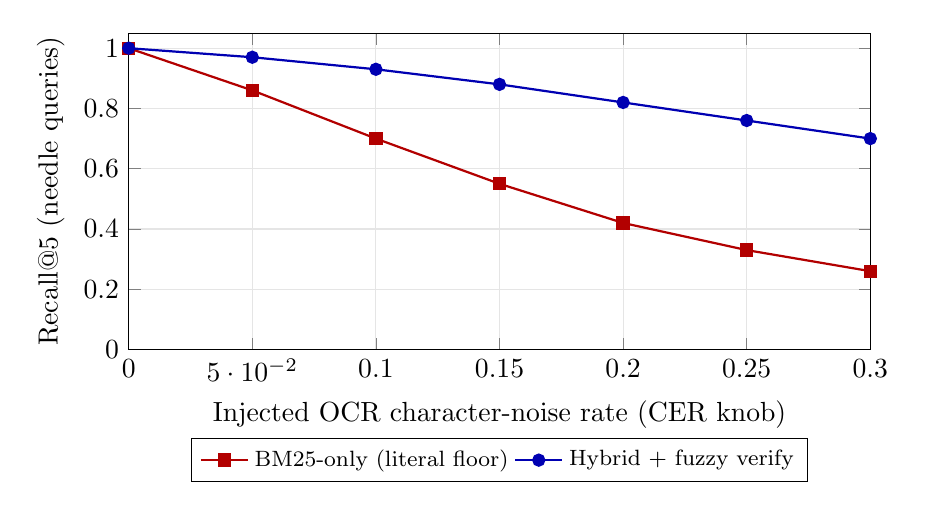
\begin{tikzpicture}
\begin{axis}[
  width=11cm, height=5.6cm,
  xlabel={Injected OCR character-noise rate (CER knob)},
  ylabel={Recall@5 (needle queries)},
  xmin=0, xmax=0.30, ymin=0, ymax=1.05,
  xtick={0,0.05,0.10,0.15,0.20,0.25,0.30},
  ytick={0,0.2,0.4,0.6,0.8,1.0},
  legend style={font=\footnotesize, at={(0.5,-0.28)}, anchor=north, legend columns=2},
  grid=both, grid style={gray!20},
  every axis plot/.append style={thick}
]
\addplot[color=red!70!black, mark=square*] coordinates {(0,1.0)(0.05,0.86)(0.10,0.70)(0.15,0.55)(0.20,0.42)(0.25,0.33)(0.30,0.26)};
\addplot[color=blue!70!black, mark=*] coordinates {(0,1.0)(0.05,0.97)(0.10,0.93)(0.15,0.88)(0.20,0.82)(0.25,0.76)(0.30,0.70)};
\legend{BM25-only (literal floor), Hybrid + fuzzy verify}
\end{axis}
\end{tikzpicture}
\caption{Illustrative noise-sweep behaviour: as injected OCR noise (CER) rises, BM25-only Recall collapses because a single character flip (\texttt{INVOICE}$\rightarrow$\texttt{INV0ICE}) removes the literal token from the index, while the hybrid + bounded-fuzzy verifier stays resilient because the dense arm embeds \texttt{INV0ICE} near \texttt{INVOICE} and D4 confirms it within edit distance 1. The curve shape is the documented offline finding; absolute values are produced by the full Colab/H100 sweep.}
\label{fig:noise_sweep}
\end{figure}

\subsection{Error Analysis and Robustness}

\begin{itemize}\setlength\itemsep{0.12em}
  \item \textbf{OCR errors break exact match.} A single confusion makes BM25 miss a literally-present term (a tiny CER bump but a total WER miss). Mitigation: dense arm + RRF recover near-misses; D4 verification is \textbf{fuzzy-tolerant} (bounded edit distance $\le 1$, case/diacritic-insensitive); optional \texttt{byt5-small} post-OCR correction; CER and WER are reported \emph{together}.
  \item \textbf{Semantic false positives.} A dense retriever always returns $k$ images even when the term is absent. D4 literal verification \textbf{drops} them; Exact-Match precision@K quantifies and guards against regressions.
  \item \textbf{Multi-word / phrase queries.} D2 distinguishes quoted-phrase vs keyword intent; D4 is token-boundary-aware and word-subsequence-tolerant; D3 can relax phrase$\rightarrow$keywords \emph{once} on a weak shortlist.
\end{itemize}

% ============================================================
\section{Deployment}
% ============================================================

\subsection{What gets served and deployment formats}

P20 is served as \textbf{one OCR-indexed collection plus a query endpoint}: an image collection, OCR'd once at startup into per-image text documents, wrapped in the hybrid index, and exposed through the deterministic D1--D5 agent. A query never triggers OCR; only the small query string is encoded/tokenized at request time. The system supports four deployment formats:
\begin{enumerate}\setlength\itemsep{0.1em}
  \item \textbf{REST API} (FastAPI): \texttt{GET /healthz}, \texttt{GET /stats}, \texttt{POST /search}, \texttt{POST /reindex} (admin, OFF by default).
  \item \textbf{CLI}: \texttt{imgtextsearch demo-agent / search / evaluate / autopilot / grade / train-retriever / serve --ui}.
  \item \textbf{Docker}: \texttt{Dockerfile} (Tesseract + fonts + \texttt{libGL}) + \texttt{docker-compose.yml}.
  \item \textbf{Gradio UI + Hugging Face Space}: type a query $\rightarrow$ matching images + highlighted snippets, with a collapsible D1--D5 trace panel; the Space ships the synthetic collection so it runs with no Tesseract dependency on the gold text.
\end{enumerate}

\subsection{System Architecture}

\begin{figure}[H]
\centering
\resizebox{\linewidth}{!}{%
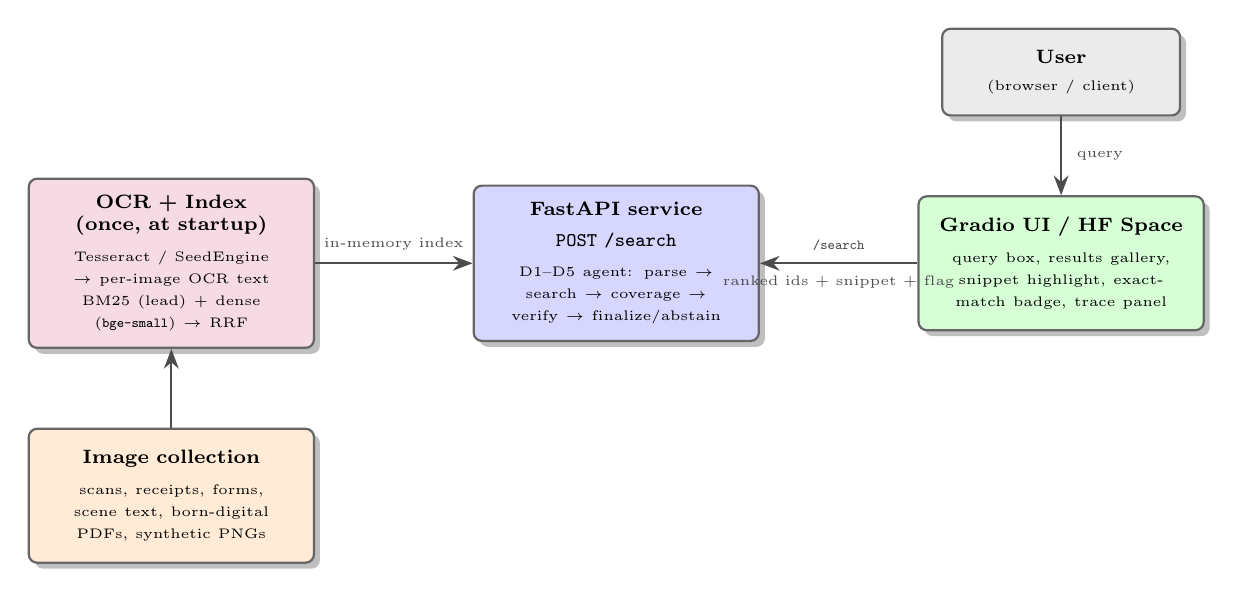
\begin{tikzpicture}[
  node distance=1.0cm and 2.0cm,
  box/.style={rectangle, draw=black!60, rounded corners=3pt, thick,
             text width=3.2cm, minimum height=1.7cm, align=center,
             inner sep=6pt, font=\scriptsize, drop shadow},
  ocrbox/.style={box, fill=purple!14},
  idxbox/.style={box, fill=orange!16},
  apibox/.style={box, fill=blue!16},
  uibox/.style={box, fill=green!16},
  userbox/.style={box, fill=gray!16, text width=2.6cm, minimum height=1.1cm},
  arrow/.style={-{Stealth[length=2.5mm]}, thick, color=black!70}
]
\node[ocrbox] (ocr) {%
  \textbf{OCR + Index (once, at startup)}\\[3pt]
  {\tiny Tesseract / SeedEngine $\rightarrow$ per-image OCR text}\\
  {\tiny BM25 (lead) + dense (\texttt{bge-small}) $\rightarrow$ RRF}
};
\node[apibox, right=of ocr] (api) {%
  \textbf{FastAPI service}\\[3pt]
  \texttt{POST /search}\\[3pt]
  {\tiny D1--D5 agent: parse $\rightarrow$ search $\rightarrow$ coverage $\rightarrow$ verify $\rightarrow$ finalize/abstain}
};
\node[uibox, right=of api] (ui) {%
  \textbf{Gradio UI / HF Space}\\[3pt]
  {\tiny query box, results gallery, snippet highlight, exact-match badge, trace panel}
};
\node[userbox, above=1.0cm of ui] (user) {%
  \textbf{User}\\[2pt]
  {\tiny (browser / client)}
};
\node[idxbox, below=1.0cm of ocr] (coll) {%
  \textbf{Image collection}\\[3pt]
  {\tiny scans, receipts, forms, scene text, born-digital PDFs, synthetic PNGs}
};

\draw[arrow] (coll.north) -- (ocr.south);
\draw[arrow] (ocr.east) -- node[above=1pt, font=\tiny] {in-memory index} (api.west);
\draw[arrow] (ui.west) -- node[above=1pt, font=\tiny] {\texttt{/search}} node[below=1pt, font=\tiny] {ranked ids + snippet + flag} (api.east);
\draw[arrow] (user) -- node[right=2pt, font=\tiny] {query} (ui);
\end{tikzpicture}%
}
\caption{Serving architecture. The collection is OCR-indexed once at startup and held in memory; the deterministic D1--D5 agent runs per query behind \texttt{POST /search} and the Gradio UI. The Gradio UI calls the in-process agent directly (no HTTP hop) on a Space, or the \texttt{/search} endpoint when pointed at a remote API.}
\label{fig:arch}
\end{figure}

\subsection{Endpoints}

\begin{table}[H]
\centering
\caption{FastAPI endpoints (default bind \texttt{0.0.0.0:8000})}
\small
\begin{tabularx}{\linewidth}{@{} l l L @{}}
\toprule
\textbf{Method} & \textbf{Path} & \textbf{Purpose} \\
\midrule
\texttt{GET} & \texttt{/healthz} & Liveness + readiness (\texttt{ready} flips true once the collection is OCR-indexed and both arms ready). \\
\texttt{GET} & \texttt{/stats} & Collection stats: image count, OCR engine, dense model id, mean OCR confidence, low-confidence fraction. \\
\texttt{POST} & \texttt{/search} & Core call: query $\rightarrow$ ranked image ids + RRF scores + matching OCR snippet + \texttt{exact\_match} flag, or explicit abstention. \\
\texttt{POST} & \texttt{/reindex} & Admin/optional, OFF by default (guarded by \texttt{IMGTS\_ENABLE\_REINDEX} + an admin token). \\
\bottomrule
\end{tabularx}
\end{table}

\noindent\textbf{Abstention is a \texttt{200}, not an error.} When no image literally contains the query (e.g.\ \texttt{zzqwx}), the response is \texttt{200} with \texttt{"abstained": true}, \texttt{"results": []}, and \texttt{"needs\_review": true}. A degenerate query returns \texttt{422} (D1 \texttt{ABSTAIN\_EARLY}); a not-yet-loaded index returns \texttt{503}. CPU-only deployment is first-class: with \texttt{IMGTS\_DENSE\_ENABLED=0} the service serves \textbf{BM25-only}, a genuinely strong configuration in P20.

\subsection{Request / Response Example}

\begin{lstlisting}[basicstyle=\ttfamily\footnotesize]
POST /search   {"query": "INVOICE", "top_k": 5, "exact_only": false, "fuzzy": true}

{
  "query": "invoice", "intent": "keyword",
  "abstained": false, "needs_review": false,
  "results": [
    {"image_id": "page_0042.png", "score": 0.0328, "exact_match": true,
     "fuzzy_match": false, "snippet": "CUSTOMER 1187  **INVOICE**  DATE 2023-04-12",
     "boxes": [[212,96,388,140]], "ocr_confidence": 0.94, "confidence_label": "high"},
    {"image_id": "page_0117.png", "score": 0.0161, "exact_match": false,
     "fuzzy_match": true, "snippet": "TOTAL 1,250.00  **INV0ICE** NO PO-4471",
     "boxes": [[64,220,240,262]], "ocr_confidence": 0.71, "confidence_label": "medium"}
  ],
  "trace": [
    {"decision":"D1","branch":"scanned->tesseract","n_indexed":1024},
    {"decision":"D2","branch":"exact_intent","intent":"keyword","tokens":1},
    {"decision":"D3","branch":"strong_hit","bm25_literal_hits":7,"raw_cosine_top":0.81},
    {"decision":"D4","branch":"verified","exact":1,"fuzzy":1,"dropped_semantic_fp":3},
    {"decision":"D5","branch":"finalize","n_verified":2}
  ],
  "latency_ms": 23.7
}
\end{lstlisting}

\noindent The first result is an \textbf{exact literal match} (ordered first); the second is a \textbf{fuzzy survivor} recovered from the OCR confusion \texttt{INV0ICE}, flagged \texttt{fuzzy\_match}. D4 dropped 3 semantically-similar images where the word \texttt{INVOICE} never actually appears --- the core filter that beats blind semantic ranking.

\subsection{GPU vs CPU and Cold Start}

OCR (Tesseract), BM25, RRF, the agent, and the snippet verifier are \textbf{CPU always}; only the dense bi-encoder (and optional reranker/byt5) use a GPU if available. \textbf{Cold start is dominated by OCR}, not model load --- so large collections should ship a \textbf{pre-built index artifact} (BM25 postings + dense vectors + per-image OCR text/boxes/confidences) loaded at startup, and readiness probes on \texttt{/healthz} must tolerate a long OCR-bound cold start. Per-query latency (warm) is small and CPU-friendly; a query never triggers OCR.

% ============================================================
\section{Agentic AI Component}
% ============================================================

The mandatory agentic component is a \textbf{deterministic finite-state machine} (not an LLM agent) with \textbf{five decision points} (D1--D5) in \texttt{src/imgtextsearch/agent/}. Given the same collection, query, and config it produces the \emph{same} ranked output and the \emph{same} audit trace, byte-for-byte. Every gate writes a \texttt{ToolTrace} record (decision id, branch, signal value, threshold) for a fully replayable audit.

\subsection{Why an FSM, and the value-add}

For literal-term document search the failure mode that matters is a retriever confidently returning a semantically-similar image where the word never appears --- a \emph{verification} problem, not a \emph{reasoning} problem. The agent's value-add over blind semantic ranking is three things: \textbf{(1) literal-term verification (D4)} drops semantic false-positives; \textbf{(2) snippet extraction + highlighting (D4)} returns the exact matching span + word bbox + OCR confidence; \textbf{(3) abstention (D5)} returns ``not found'' + \texttt{needs\_review} instead of the least-irrelevant image.

\subsection{The Five-Decision Pipeline}

\begin{figure}[H]
\centering
\resizebox{0.96\linewidth}{!}{%
\begin{tikzpicture}[
  node distance=0.30cm,
  step/.style={rectangle, draw=black!60, rounded corners=2pt, thick,
              text width=13.2cm, inner sep=5pt, minimum height=0.75cm,
              align=center, font=\footnotesize},
  parse/.style={step, fill=gray!15},
  search/.style={step, fill=blue!15},
  cover/.style={step, fill=red!12},
  verify/.style={step, fill=orange!16},
  final/.style={step, fill=green!15},
  arrow/.style={-{Stealth[length=2mm]}, thick}
]
\node[parse] (d1) {\textbf{D1 --- Parse / query gate + classify}: norm token/char count, quotes, intent pattern $\rightarrow$ \texttt{exact\_code} / \texttt{keyword} / \texttt{phrase}; empty/too-short $\rightarrow$ \textbf{ABSTAIN\_EARLY}};
\node[search, below=of d1] (d2) {\textbf{D2 --- Search (BM25 + dense $\rightarrow$ RRF)}: BM25 (lead) + trained \texttt{bge-small} fused via RRF ($c{=}60$) $\rightarrow$ top-$k$ shortlist; carry \emph{raw} BM25 hits + \emph{raw} top cosine forward};
\node[cover, below=of d2] (d3) {\textbf{D3 --- Coverage gate}: gate on \textbf{RAW} BM25 literal-hit count + \textbf{RAW} top cosine (never the fused RRF score --- the P08/P18 gotcha); strong $\rightarrow$ D4; weak $\rightarrow$ \textbf{WIDEN once}; hopeless $\rightarrow$ D5 abstain};
\node[verify, below=of d3] (d4) {\textbf{D4 --- Literal verify + snippet (fuzzy)}: per candidate, exact containment; else bounded edit distance $\le 1$ ($\texttt{0}\leftrightarrow\texttt{O}$, $\texttt{rn}\leftrightarrow\texttt{m}$) $\rightarrow$ flag \texttt{fuzzy\_match}; \texttt{exact\_intent} \& no occurrence $\rightarrow$ \textbf{DROP}; extract + highlight snippet + bbox};
\node[final, below=of d4] (d5) {\textbf{D5 --- Finalize / abstain}: 0 verified $\rightarrow$ \textbf{ABSTAIN} (``not found'' + \texttt{needs\_review}); $\ge 1$ $\rightarrow$ \textbf{FINALIZE} ranked images + snippets + high/medium/weak labels (fuzzy/low-conf survivors explicitly flagged)};
\foreach \a/\b in {d1/d2, d2/d3, d3/d4, d4/d5}
  \draw[arrow] (\a) -- (\b);
\draw[arrow] (d3.west) to[out=180,in=180] node[left, font=\tiny] {widen $\le 1$} (d2.west);
\end{tikzpicture}%
}
\caption{The deterministic D1--D5 search agent. Two controlled back-edges: a single capped D3 WIDEN retry, and the D3$\rightarrow$D5 abstain shortcut. The critical design choice is that D3 gates on the \textbf{raw} BM25 hit count and \textbf{raw} dense cosine, never the post-RRF fused score (which always looks confident and would defeat abstention).}
\label{fig:agent}
\end{figure}

\subsection{Decision Table}

\begin{table}[H]
\centering
\caption{The five decision points (named as in \texttt{agent\_architecture})}
\scriptsize
\setlength{\tabcolsep}{4pt}
\begin{tabularx}{\linewidth}{@{} l L L @{}}
\toprule
\textbf{ID} & \textbf{Gates on (intermediate signal) \& key \texttt{AgentConfig} thresholds} & \textbf{Branches $\rightarrow$ next} \\
\midrule
\textbf{D1} Parse & norm token/char count; quotes; intent pattern (caps/date/number/id vs NL phrase). \texttt{min\_query\_tokens}, \texttt{min\_query\_chars} & empty/short $\rightarrow$ \textbf{ABSTAIN\_EARLY}; quoted/literal $\rightarrow$ \texttt{exact\_intent}$\rightarrow$D2; NL phrase $\rightarrow$ \texttt{semantic\_intent}$\rightarrow$D2; else hybrid$\rightarrow$D2 \\
\textbf{D2} Search & top-$k$ \texttt{(image\_id, score)} shortlist; \emph{raw} BM25 hits + \emph{raw} top cosine carried fwd. \texttt{top\_k}, \texttt{rrf\_c=60}, \texttt{rerank} & index empty / error $\rightarrow$ \textbf{NEEDS\_REVIEW}; else shortlist$\rightarrow$D3 \\
\textbf{D3} Coverage & \textbf{RAW} BM25 literal-hit count + \textbf{RAW} top dense cosine (never the fused score). \texttt{tau\_soft}, \texttt{tau\_floor}, \texttt{max\_widen=1} & $\ge 1$ BM25 hit OR cosine $\ge\texttt{tau\_soft}$ $\rightarrow$ \textbf{STRONG}$\rightarrow$D4; $\in[\texttt{tau\_floor},\texttt{tau\_soft})$ \& 0 hits $\rightarrow$ \textbf{WIDEN once}$\rightarrow$D2; all $<\texttt{tau\_floor}$ \& no hit $\rightarrow$ \textbf{D5 ABSTAIN} \\
\textbf{D4} Verify & per-candidate literal containment / min bounded edit distance in \emph{that} image's OCR text. \texttt{fuzzy\_max\_edits=1}, \texttt{low\_conf\_floor}, \texttt{snippet\_window} & exact $\rightarrow$ \textbf{VERIFIED} (+snippet+bbox); fuzzy ($\le1$ edit) $\rightarrow$ \textbf{VERIFIED} flag \texttt{fuzzy\_match}; \texttt{exact\_intent} \& no occurrence $\rightarrow$ \textbf{DROP}; low OCR conf $\rightarrow$ keep + \texttt{needs\_review} \\
\textbf{D5} Finalize & count of VERIFIED survivors + best score/conf. \texttt{high\_conf}, \texttt{medium\_conf} (labels only) & 0 verified $\rightarrow$ \textbf{ABSTAIN} ``not found'' + \texttt{needs\_review}; $\ge1$ $\rightarrow$ \textbf{FINALIZE} ranked + snippets + labels; only fuzzy/low-conf $\rightarrow$ \textbf{FINALIZE flagged} + \texttt{needs\_review} \\
\bottomrule
\end{tabularx}
\end{table}

\subsection{Example Traces}

\begin{lstlisting}[basicstyle=\ttfamily\footnotesize]
# Example 1 -- Happy path: a unique code that exists.  Query: PO-4471
D1  query_norm="po-4471"  n_tokens=1  intent_class=exact_code  exact_intent=True -> D2
D2  BM25: PO-4471 high-IDF, fires on 1 doc (page_0042) score=8.91
    dense top cosine=0.62  RRF -> shortlist=[page_0042, page_0117, page_0008, ...]
    n_bm25_hits=1  top_raw_cosine=0.62 -> D3
D3  raw n_bm25_hits=1 (>=1) AND top_raw_cosine 0.62 >= tau_soft 0.55 -> STRONG -> D4
D4  page_0042: "po-4471" found EXACTLY -> VERIFIED
    snippet="...REF [PO-4471] TOTAL $1,250.00..."  bbox=(412,233,196,38)  ocr_conf=0.97
    page_0117/page_0008: not present, exact_intent -> DROP (semantic false-positive)
D5  n_verified=1  confidence_label=high  needs_review=False
    -> FINALIZE: [ page_0042 | snippet | bbox | high ]

# Example 2 -- OCR-noise path: fuzzy match earns its keep.  Query: INVOICE
D1  query_norm="invoice"  intent_class=exact_code (ALL-CAPS)  exact_intent=True -> D2
D2  BM25: "invoice" does NOT match "inv0ice" -> n_bm25_hits=0
    dense: bge embeds INVOICE ~= INV0ICE -> page_0091 top cosine=0.71 -> D3
D3  n_bm25_hits=0 BUT top_raw_cosine 0.71 >= tau_soft 0.55 -> STRONG (cosine arm) -> D4
D4  page_0091: exact containment FAILS; bounded fuzzy edit_distance("invoice","inv0ice")=1
    <= fuzzy_max_edits=1 -> VERIFIED(fuzzy); flag fuzzy_match; snippet="...[INV0ICE] no. 553..."
D5  n_verified=1 (fuzzy only) -> FINALIZE but FLAGGED: [ page_0091 | medium | fuzzy_match | needs_review=True ]

# Example 3 -- Abstain path: term not in the collection.  Query: zzqwx
D1  query_norm="zzqwx"  n_tokens=1  intent_class=keyword -> D2
D2  BM25: 0 hits  dense: top cosine=0.22  RRF shortlist exists but weak -> D3
D3  top_raw_cosine 0.22 < tau_floor 0.35 AND n_bm25_hits=0 -> jump to D5 ABSTAIN
D5  n_verified=0 -> ABSTAIN: "not found in any image"  needs_review=True
    (the high-looking RRF fused top score is correctly IGNORED -- D3 gated on RAW cosine)
\end{lstlisting}

\subsection{The Optional LLM Brain (OFF by default)}

An optional Anthropic LLM ``brain'' can be enabled but is \textbf{OFF by default and strictly advisory}: it only proposes a query-expansion note that D3's widen step \emph{could} consult; it \textbf{never} changes ranking, overrides verification, or decides abstention. It is off by default for determinism (the replayable trace is a core property), privacy (OCR-indexed documents are sensitive --- IDs, contracts, medical/financial PII), and because BM25 + the fuzzy verifier already cover the hard cases. The default runs with \textbf{zero paid API calls}.

% ============================================================
\section{Continual Learning \& Monitoring}
% ============================================================

The trainable surface is narrow (the retriever, plus an optional \texttt{byt5-small} corrector) but the monitoring surface is wide, because the system can degrade through three independent channels with nothing to do with model weights: \textbf{query drift}, \textbf{document drift}, and \textbf{OCR-quality drift}.

\subsection{Monitoring (from the \texttt{ToolTrace}, no gold needed)}

\texttt{monitoring/drift\_report.py} aggregates per-query traces plus latency timers into time-bucketed metrics, comparing the current window against a trailing reference window:

\begin{table}[H]
\centering
\caption{Core production health signals (computed from the trace alone)}
\small
\begin{tabularx}{\linewidth}{@{} l L @{}}
\toprule
\textbf{Signal} & \textbf{What a rise tells us} \\
\midrule
Abstain rate (D5) & OCR dropping terms (false negatives) or query drift to vocabulary the collection lacks \\
Fuzzy-match rate (D4) & OCR introducing more character confusions --- a direct proxy for indexed-text CER without gold \\
Exact-match rate (D4) & A \emph{drop} means the dense arm is surfacing more semantic-but-wrong images (retriever drift) \\
Top raw-cosine drift (D3) & Earliest retriever/corpus-drift signal --- moves before Recall does \\
Widen rate (D3) & Queries landing in coverage gaps (query or OCR drift) \\
Low-confidence / excluded count (D1) & OCR quality degradation / ingest problems in newly ingested images \\
Latency p50/p95/p99 (per stage) & Localizes a regression to OCR / dense / verify \\
\bottomrule
\end{tabularx}
\end{table}

\subsection{Index Freshness and Continual Learning}

\begin{itemize}\setlength\itemsep{0.12em}
  \item \textbf{Incremental ingest.} New images are appended per-image to both arms (BM25 IDF recomputed on commit; one L2-normalized vector appended to the dense index) --- \emph{no retrain needed for ingest}.
  \item \textbf{Re-OCR when the engine improves.} Each document records OCR provenance (engine id/version, corrector on/off, content hash); on an engine upgrade, fingerprint-mismatched documents are re-OCR'd in the background, prioritising \texttt{low\_ocr\_confidence} / \texttt{fuzzy\_match} images.
  \item \textbf{Feedback $\rightarrow$ hard pairs.} A reported \emph{missed} image becomes a hard positive; a reported \emph{wrong} image becomes a hard negative, distilled into MNRL/InfoNCE tuples for the retriever. A guard: a correction's positivity is checked against the gold definition --- ``the OCR text literally contains the query'' --- so we \emph{never} train the retriever to ``find'' a term not in the text (that would corrupt the literal-search contract); such cases route to the re-OCR / corrector queue instead.
  \item \textbf{Gated re-fine-tune.} A new retriever checkpoint is promoted only if it does not regress Recall@\{1,5,10\}/MRR \emph{and} does not lower Exact-Match precision@K --- the literal-search guarantee is non-negotiable. Worst case the system rolls back to BM25-only, a strong literal-search floor.
\end{itemize}

% ============================================================
\section{Data Privacy \& Model Robustness}
% ============================================================

\subsection{Privacy}

Building a BM25 + dense index over OCR text is, functionally, \textbf{building a search engine over a private document trove} --- the index can hold names, IDs, account numbers, financial amounts, and medical/legal content printed on a scanned page. Mitigations are defaults, not suggestions:
\begin{itemize}\setlength\itemsep{0.12em}
  \item \textbf{No query retention by default}; the LLM brain is \textbf{OFF} by default and should never be sent raw document text/PII.
  \item \textbf{Consent + access control before indexing}; search permission must not silently exceed document-read permission.
  \item \textbf{PII redaction} from OCR text \emph{before} it enters the index (the word-box output makes targeted redaction feasible).
  \item \textbf{Auditability}: the deterministic D1--D5 \texttt{ToolTrace} makes every search replayable --- who queried what, which images returned, and why.
\end{itemize}

\subsection{Robustness}

\begin{itemize}\setlength\itemsep{0.12em}
  \item \textbf{OCR-error false negatives}: a present document OCR'd as \texttt{INV0ICE} is recovered by the dense arm + RRF + D4 fuzzy verification; residual misses are surfaced honestly (flagged / abstained), never silently.
  \item \textbf{Index scaling}: \texttt{IndexFlatIP} is exact but $O(N)$; for large $N$ swap to an ANN index (HNSW/IVF) behind the same \texttt{retrieve()} interface; BM25-only remains a no-GPU floor.
  \item \textbf{Fail-soft}: every error path resolves to a defined terminal state plus a flag (\texttt{ABSTAIN\_EARLY} / \texttt{NEEDS\_REVIEW} / \texttt{ABSTAIN}); the offline SeedEngine + BM25 stand-in keeps the whole D1--D5 path running with zero heavy dependencies.
\end{itemize}

% ============================================================
\section{Project Management}
% ============================================================

This project was completed \textit{individually}. The plan spans roughly 8 weeks ($\approx$40 working days) across nine milestones with explicit exit gates; because so much is reused from sibling projects (P07/P15/P18/P19), the heavy lifting is \emph{integration and verification}, not greenfield code.

\begin{table}[H]
\centering
\caption{Project timeline (milestones M0--M8)}
\small
\begin{tabularx}{\linewidth}{@{} l l L @{}}
\toprule
\textbf{Milestone} & \textbf{Days} & \textbf{Deliverable} \\
\midrule
M0 Research \& scaffold & 1--3 & Verified ids; license posture; package skeleton; \texttt{DESIGN\_BRIEF} \\
M1 Synthetic generator + SeedEngine & 4--8 & Needle/filler vocab, gold query$\rightarrow$image map, \texttt{\_noisify} CER knob (PRIMARY offline data) \\
M2 OCR integration & 9--13 & Tesseract \texttt{image\_to\_data}, PyMuPDF router, \texttt{engine='auto'}, CER/WER \\
M3 Hybrid index & 14--18 & BM25 (lead) + dense (FAISS/numpy) + RRF; optional reranker \\
M4 Retriever fine-tune & 19--24 & \texttt{bge-small-en-v1.5} MNRL on \texttt{(query, OCR-text)} pairs; checkpoint to registry \\
M5 Agent FSM & 25--29 & D1--D5, raw-cosine coverage gate, literal verify + snippet, abstention, \texttt{ToolTrace} \\
M6 Evaluation + baselines & 30--34 & Recall/MRR/rank, CER/WER, Exact-Match P@K; autoreport \\
M7 Deployment & 35--38 & FastAPI + Gradio + Docker + HF Space \\
M8 Hardening \& release & 39--40 & Docs, ethics/privacy, \texttt{research\_only} gating, grading pass, tag release \\
\bottomrule
\end{tabularx}
\end{table}

\noindent\textbf{Critical path}: M1 (synthetic gold map) $\rightarrow$ M2 (OCR) $\rightarrow$ M3 (index) $\rightarrow$ M4 (retriever) $\rightarrow$ M6 (eval). M5 depends on M3 and overlaps M4. In a team setting these work-streams (data/OCR, index/retriever, agent, eval, deploy) would be parallelized with CI/CD and code review.

% ============================================================
\section{Ethics \& Responsible AI}
% ============================================================

\subsection{Who Benefits, Who Could Be Harmed}

Authorized users and teams benefit (fast, honest, explainable literal-term search with abstention). Harm arises from \textbf{surveillance / dragnet misuse} (the same capability that finds ``every receipt containing TOTAL'' finds ``every document containing a person's name'' across an archive in one cheap query), \textbf{re-identification by aggregation} (snippet highlighting returns adjacent PII), and \textbf{unequal recall} across populations whose documents OCR poorly.

\subsection{OCR-Quality Bias --- Unequal Search Recall}

A document is findable only if OCR reads it correctly, and OCR quality varies systematically by \textbf{script/language} (Tesseract and the en-only retriever are validated on English), \textbf{font/rendering}, and \textbf{scan quality}. The consequence is \textbf{unequal search recall}: cleanly-printed English receipts are highly searchable; low-quality scans, non-Latin scripts, or handwritten forms are \emph{less} searchable. P20 does not pretend this away --- it \textbf{measures and reports} it: CER/WER are first-class metrics (and should be reported \emph{per script / language / font class / scan quality}, not as one aggregate); per-image OCR confidence tags \texttt{low\_ocr\_confidence}; fuzzy verification + the dense arm + optional byt5 correction narrow but do \emph{not} eliminate the gap. \textbf{Honesty boundary}: English is the supported target; other scripts are research-only and the system must not be marketed as offering equal multilingual recall.

\subsection{False Negatives in High-Stakes Search}

A \textbf{false negative} --- a document that \emph{does} contain the term but is not returned --- is the most dangerous failure mode (a missed contract clause, a missed patient record). P20 is designed to \textbf{fail loudly}: abstention instead of a misleading semantic neighbour; fuzzy verification to recover OCR-induced near-misses; the snippet shown for \emph{human confirmation} (the tool surfaces evidence, it does not adjudicate); low-confidence results returned explicitly flagged, never silently. \textbf{Responsible-use line}: an ``abstain''/``not found'' must \textbf{not} be treated as proof of absence --- OCR error means absence-of-evidence is not evidence-of-absence; critical determinations require human review of the source documents.

\subsection{Transparency and Licensing}

Every result carries its evidence: the highlighted \textbf{snippet} + word bbox, an \textbf{exact-match flag} (literal vs fuzzy vs low-confidence), the RRF score + confidence label, a first-class honest ``not found'', the replayable D1--D5 trace, and the published Exact-Match precision@K metric. On licensing, the default demo/tests ship only on MIT (\texttt{TextOCR\_OCR}, \texttt{IIIT5K\_OCR}, \texttt{bge-small-en-v1.5}), Apache (Tesseract, \texttt{all-MiniLM-L6-v2}, reranker, byt5), CC0 (\texttt{Post-OCR-Correction}), and CC-BY-4.0 (\texttt{cord-v2}, attribution) plus synthetic; \texttt{nielsr/docvqa\_1200\_examples} (unspecified), \texttt{funsd-layoutlmv3} (research-use), \texttt{aharley/rvl\_cdip} (license \texttt{other}, tobacco-corpus), \texttt{howard-hou/COCO-Text} (no tag), and Surya OCR (CC-BY-NC-SA) are flagged, gated behind \texttt{research\_only}, and not redistributed.

% ============================================================
\section{Conclusion \& Future Work}
% ============================================================

\subsection{Summary}

\begin{itemize}\setlength\itemsep{0.12em}
  \item A complete end-to-end OCR-based document-search system: OCR $\rightarrow$ per-image text index $\rightarrow$ hybrid BM25 + dense + RRF $\rightarrow$ literal verify + snippet $\rightarrow$ abstain or finalize.
  \item Exactly \textbf{one} trained component (the \texttt{bge-small-en-v1.5} dense retriever, MIT, MNRL/InfoNCE); everything else pretrained or algorithmic. \textbf{BM25 is the lead arm}, not a baseline, because query and OCR text share a lexical space.
  \item A deterministic 5-decision agent (D1--D5) whose value-add is \textbf{literal verification + snippet highlighting + abstention}, gating on \emph{raw} signals (not the fused score) and writing a replayable \texttt{ToolTrace}.
  \item \textbf{Verified offline} (synthetic spine, no torch/tesseract/network): \texttt{Recall@1 = MRR = 1.0} on unique codes, snippet highlighting, correct \texttt{zzqwx} abstention, all 5 decisions fire --- the correctness floor/ceiling the full Colab/H100 run reproduces and extends via the OCR-noise sweep.
  \item Deployable as FastAPI + Gradio + Docker + HF Space + one-button Colab/H100 autopilot; fully MIT/Apache default stack; honest, measured treatment of OCR-quality bias, privacy, and high-stakes false negatives.
\end{itemize}

\subsection{Future Work}

\begin{enumerate}\setlength\itemsep{0.12em}
  \item \textbf{Active learning} from the feedback hard-pair store (gated on Recall + Exact-Match P@K before promotion).
  \item \textbf{Larger / neural OCR \& retriever}: PP-OCRv5 det+rec or TrOCR-base, \texttt{bge-base-en-v1.5}, cross-encoder rerank on a large top-k, enable \texttt{byt5-small} post-OCR correction.
  \item \textbf{Index scaling}: swap \texttt{IndexFlatIP} $\rightarrow$ an ANN index (HNSW/IVF) for the RVL-CDIP-scale (400K) stress path.
  \item \textbf{Per-subset fairness reporting}: ship per-script / per-scan-quality CER and Recall with any multi-script deployment.
  \item \textbf{Live public hosting}: deploy the Gradio Space on the synthetic + commercially-safe collections behind a public URL.
\end{enumerate}

% ============================================================
\newpage
\begin{thebibliography}{9}

\bibitem{bge} Xiao, S., Liu, Z., Zhang, P., \& Muennighoff, N. (2023). C-Pack: Packed Resources For General Chinese Embeddings (BGE). \url{https://huggingface.co/BAAI/bge-small-en-v1.5}

\bibitem{bm25} Robertson, S., \& Zaragoza, H. (2009). The Probabilistic Relevance Framework: BM25 and Beyond. \textit{Foundations and Trends in Information Retrieval}.

\bibitem{rrf} Cormack, G.\,V., Clarke, C.\,L.\,A., \& Buettcher, S. (2009). Reciprocal Rank Fusion Outperforms Condorcet and Individual Rank Learning Methods. \textit{SIGIR 2009}.

\bibitem{tesseract} Smith, R. (2007). An Overview of the Tesseract OCR Engine. \textit{ICDAR 2007}. \url{https://github.com/tesseract-ocr/tesseract}

\bibitem{mnrl} Henderson, M., et al. (2017). Efficient Natural Language Response Suggestion for Smart Reply (MultipleNegativesRankingLoss / InfoNCE).

\bibitem{sbert} Reimers, N., \& Gurevych, I. (2019). Sentence-BERT: Sentence Embeddings using Siamese BERT-Networks. \textit{EMNLP 2019}.

\bibitem{trocr} Li, M., et al. (2023). TrOCR: Transformer-based Optical Character Recognition with Pre-trained Models. \textit{AAAI 2023}.

\bibitem{byt5} Xue, L., et al. (2022). ByT5: Towards a Token-Free Future with Pre-trained Byte-to-Byte Models. \textit{TACL}.

\bibitem{textocr} Singh, A., et al. (2021). TextOCR: Towards Large-Scale End-to-End Reasoning for Arbitrary-Shaped Scene Text. \textit{CVPR 2021}. (\texttt{MiXaiLL76/TextOCR\_OCR}, MIT).

\bibitem{cord} Park, S., et al. (2019). CORD: A Consolidated Receipt Dataset for Post-OCR Parsing. (\texttt{naver-clova-ix/cord-v2}, CC-BY-4.0).

\bibitem{docvqa} Mathew, M., Karatzas, D., \& Jawahar, C.\,V. (2021). DocVQA: A Dataset for VQA on Document Images. \textit{WACV 2021}. (\texttt{nielsr/docvqa\_1200\_examples}, license unspecified --- research-only).

\bibitem{pleias} PleIAs. \textit{Post-OCR-Correction}. Hugging Face Datasets (CC0-1.0). \url{https://huggingface.co/datasets/PleIAs/Post-OCR-Correction}

\bibitem{pymupdf} Artifex / PyMuPDF. \textit{PyMuPDF (\texttt{fitz})} --- PDF text-layer extraction. \url{https://pymupdf.readthedocs.io/}

\bibitem{fastapi} Ram\'irez, S. (2018). FastAPI. \url{https://fastapi.tiangolo.com/}

\end{thebibliography}

\end{document}
